\documentclass[UTF8]{ctexart}
\usepackage{graphicx}
\usepackage{amsmath}
\usepackage{cite}
\usepackage{mathtools}
\usepackage[a4paper,left=2.5cm,right=2.5cm,top=3cm,bottom=3cm]{geometry}
\title{液体表面张力系数的测定:实验报告}
\author{禤科材 PB20030874 20级14系 707组 1号台}
\date{\today}
\bibliographystyle{plain}

\begin{document}
    \maketitle
    \tableofcontents

    \section{实验目的}
    
        \begin{center}
            学习焦利氏秤的设计原理,并使用焦利氏秤测量液体的表面张力系数
        \end{center}

    \section{实验原理}

    \begin{center}
        \emph{\zihao{-4}表面张力的产生与作用规律}\\[0.4cm]
    \end{center}
    

    液体具有尽量缩小其表面的趋势,物理学家把这种沿着表面的、收缩液面的力称为表面张力\cite{jiangyi}

    液体表面层内的分子所处的环境跟液体内部的分子是不同的。
表面层内的分子合力垂直于液面并指向液体内部,所以分子有从液面挤入液体内部的倾向。
想象在液面上划一条直线,表面张力就表现为直线两旁的液膜以一定的拉力的相互作用。
拉力$F$存在于表面层,方向与直线垂直,大小与直线的长度$l$成正比:

\begin{equation}
    F=\sigma l
\end{equation}
式中$\sigma $称为表面张力系数,它是液体的成分、纯度、浓度以及温度的函数。
查询资料可知,密度小而易挥发的液体张力系数$\sigma $小;
液体中掺入某些杂质还可以改变张力系数$\sigma $\\[0.4cm]

\begin{center}
    \emph{\zihao{-4}拉脱法原理}\\[0.4cm]
\end{center}

\begin{figure}[ht]
    \centering 
    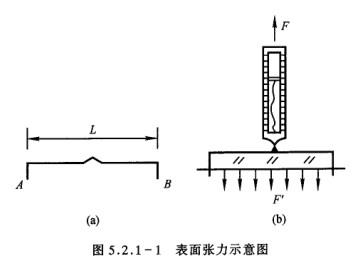
\includegraphics[width=6cm]{图片1.jpg}
\end{figure}

把金属丝AB弯成如图5.2.1-1(a)\cite{dawushiyan}所示的形状,并将其悬挂在灵敏的测力计上,然后把它浸到液体中。
当缓缓提起测力计时,金属丝就会拉出一层与液体相连的液膜,由于表面张力的作用,测力计的读数逐渐达到一临界值$F$,
由于液膜有两个表面,若每个表面的力为$F’$,则根据牛顿第一定律:
\begin{equation}
    F'=\frac{F-mg}{2}
\end{equation}

测定表面张力系数的关键是测量表面张力$F’$
用普通的弹簧是很难得知液膜即将破裂时的受力情况,而焦利氏秤的独特设计则克服了这一困难。\\[0.4cm]

\begin{center}
    \emph{\zihao{-4}焦利氏秤的结构与使用注意事项} \\[0.4cm]
\end{center}

焦利氏秤由固定在底座上的秤框、可升降的金属杆和锥形弹簧秤等部分组成。
在秤框上固定有下部可调节的载物平台、作为平衡参考点用的玻璃管和作弹簧伸长量读数用的游标;升降杆位于秤框内部,其上部有刻度,用以读出高度。
框顶端带有螺旋,供固定锥形弹簧秤用,杆的上升和下降由位于秤框下端的升降钮控制;锥形弹簧秤由锥形弹簧、带小镜子的金属挂钩及砝码盘组成。带镜子的挂钩从平衡指示玻璃管内穿过,且不与玻璃管相碰。

为了保证弹簧下端的位置是固定的,必须三线对齐。即玻璃圆筒$E$上的刻线、
小平面镜上的刻线、$E$上的刻线在小平面镜中的像三者始终重合。
在力$F$作用下弹簧伸长$\varDelta l$,根据胡克定律,在弹性限度内:

\begin{equation}
    F = k \varDelta l
\end{equation}

将一系列已知重量的砝码加在砝码盘中,分别测出弹簧的伸长量,使用最小二乘法,由上式即可计算该弹簧的劲度系数$k$
值,由$k$值就可测所受外力$F$

    \section{实验步骤}

    \emph{\\[0.02cm]\zihao{-4}1.确定焦利氏秤上锥形弹簧的劲度系数}

    (1)把锥形弹簧,带小镜子的挂钩和小砝码盘依次安装到秤框内的
    金属杆上。调节支架底座的底脚螺丝,使秤框竖直,小镜子应正好位
    于玻璃管中间,挂钩上下运动时不致与管摩擦。

    (2) 逐次在砝码盘内放入砝码,每次增量 0.5g 的砝码,从 0.5g~5g 范围内增加。每次操
    作都要调节升降钮,做到三线对齐。记录升降杆的位置读数。用最小二乘法计算出弹簧的劲度系数。

    \emph{\\[0.02cm]\zihao{-4}2.用金属圈测量自来水的表面张力系数}

    (1) 用直尺测量金属圈的直径和金属圈两脚之间的距离$d$

    (2) 取下砝码,在砝码盘下挂上已清洗过的金属圈,仍保持三线对齐,记下此时升降杆读数$l_0$

    (3) 把盛有自来水的烧杯放在焦利氏秤台上,调节平台的微调螺丝和升降钮,使金属圈浸入水面以下

    (4) 缓慢地旋转平台微调螺丝和升降钮,注意烧杯下降和金属杆上升时,始终保持三线对齐。当液膜刚要破裂时,记下金属杆的读数。
    测量$5$次,取平均,计算自来水的表面张力系数和不确定度

    \emph{\\[0.02cm]\zihao{-4}3.用金属丝测量洗洁精的表面张力系数}

    (1) 用直尺测量金属丝两脚之间的距离 s

    (2) 取下砝码,在砝码盘下挂上已清洗过的金属丝,仍保持三线对齐,记下此时升降杆
    读数 ;然后重复上述 2 中的步骤(3)和(4)步骤即可

    

    \section{实验记录}

    \begin{figure}[ht]
        \centering 
        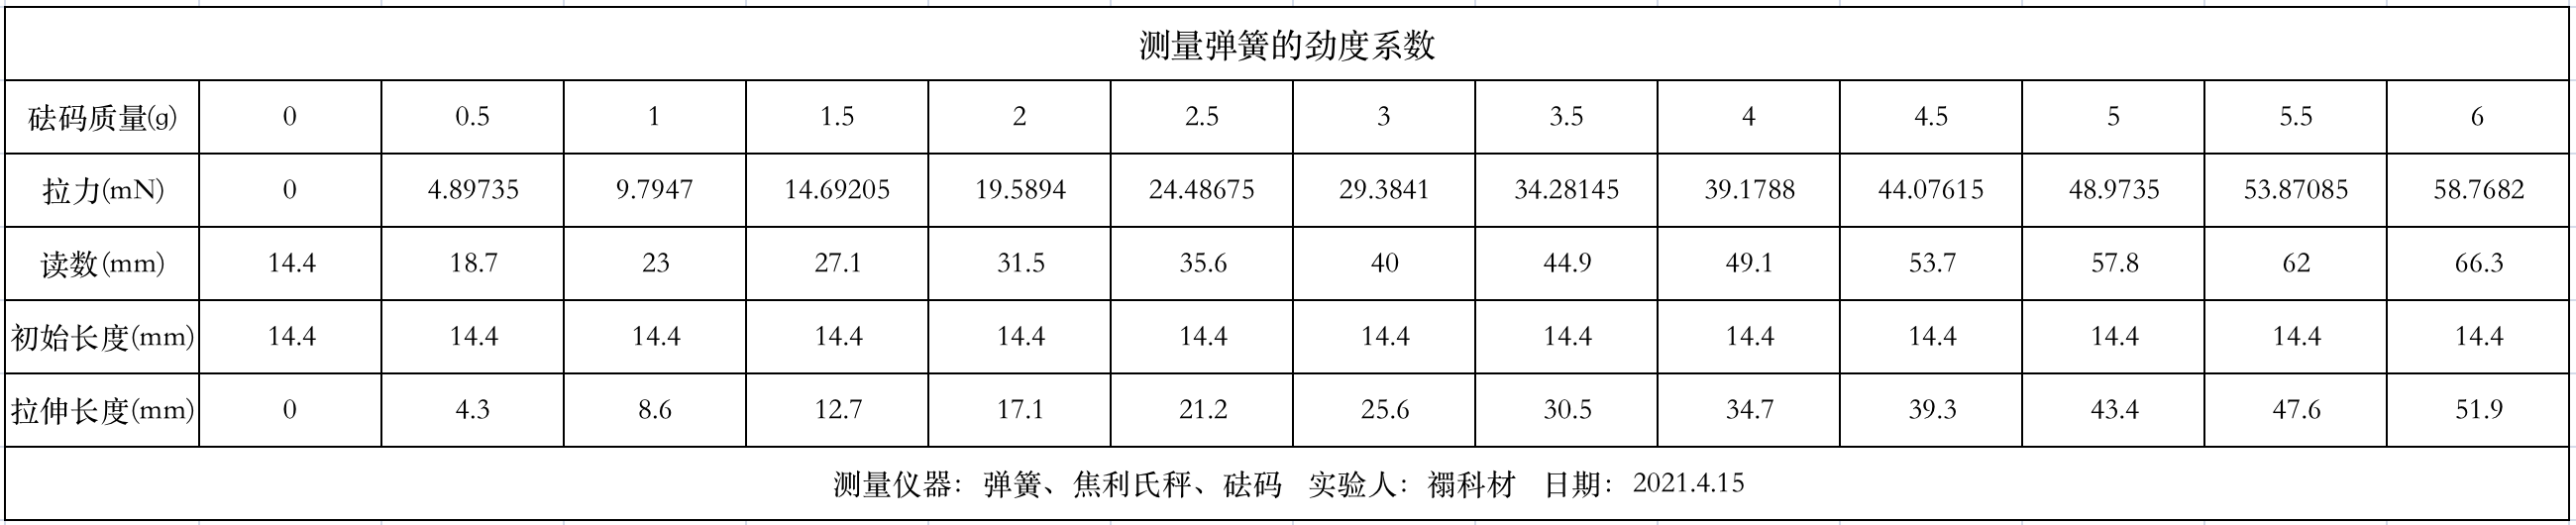
\includegraphics[width=16cm]{劲度系数.png}
    \end{figure} 

    \begin{figure}[ht]
        \centering 
        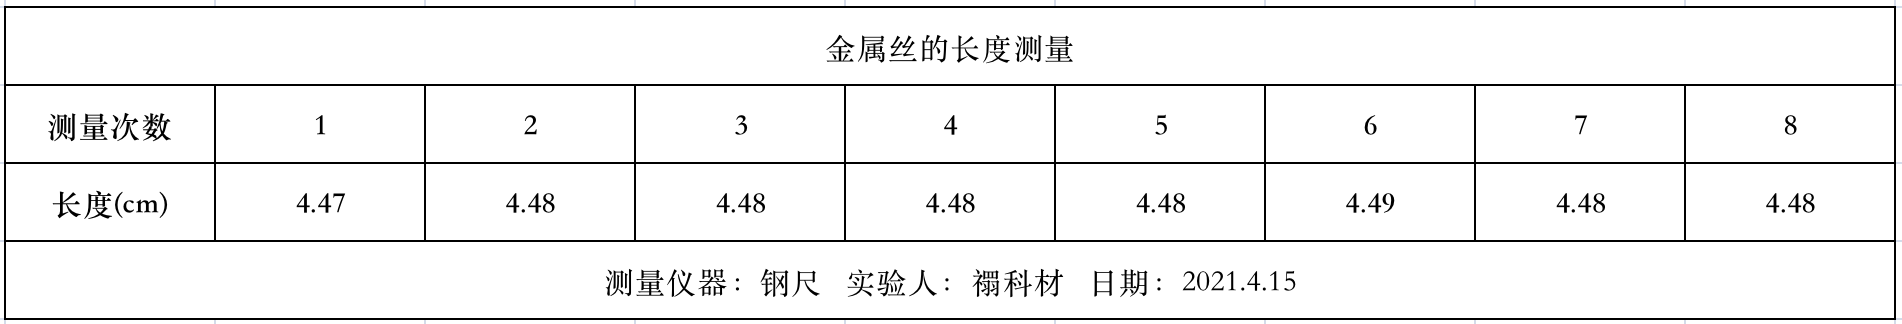
\includegraphics[width=14cm]{金属丝长度.png}
    \end{figure} 

    \begin{figure}[ht]
        \centering 
        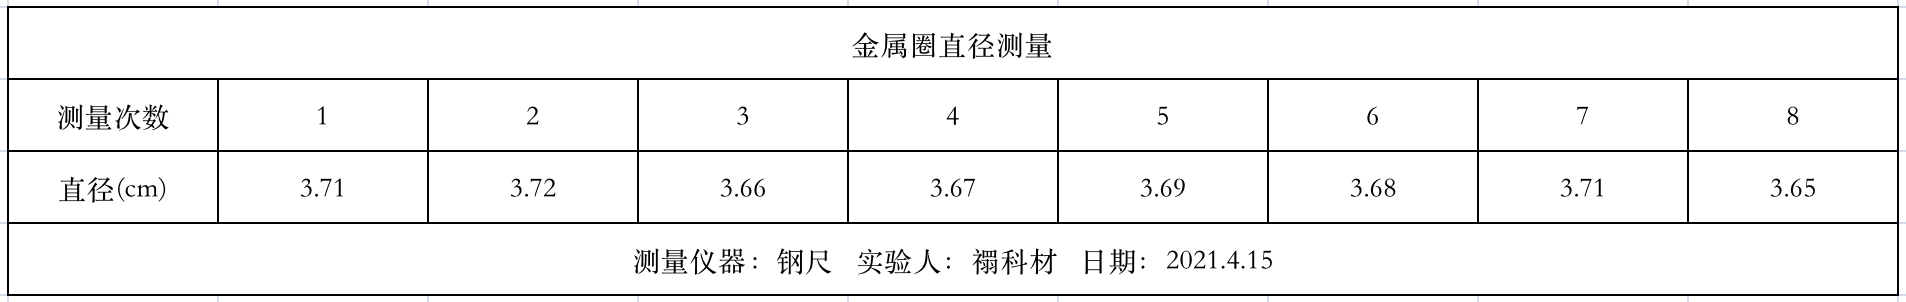
\includegraphics[width=14cm]{金属圈直径.png}
    \end{figure}


    \begin{center}
        \emph{\\[0.01cm]\zihao{-4}金属丝测量表面张力}
    \end{center}

    \begin{figure}[ht]
        \centering 
        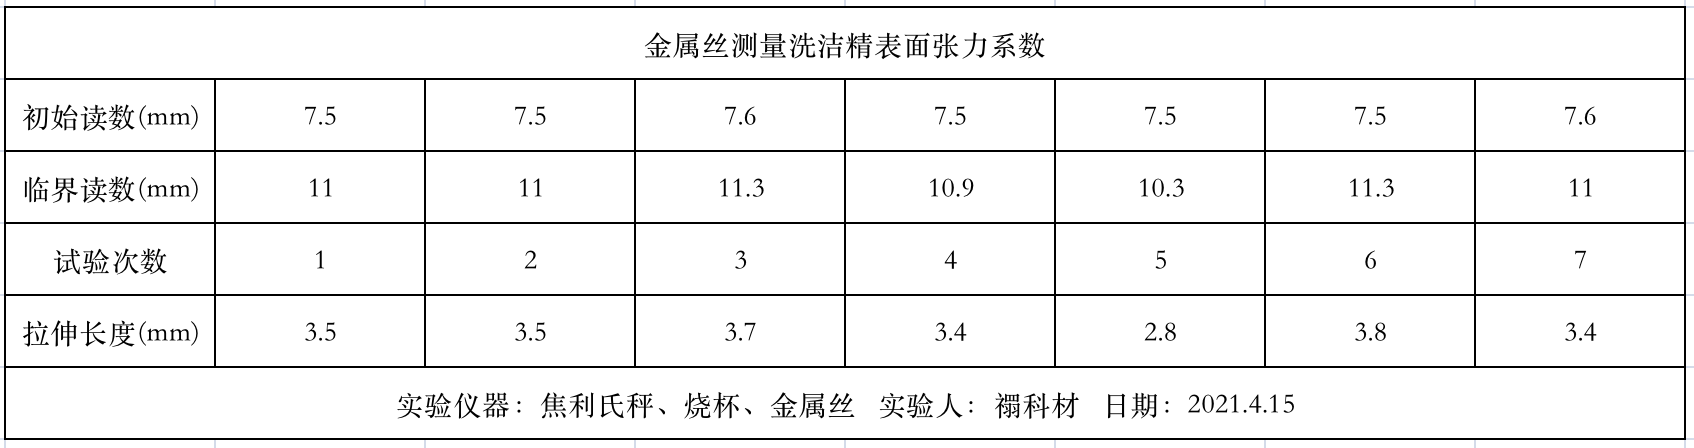
\includegraphics[width=13cm]{洗洁精.png}
    \end{figure}

    \begin{figure}[ht]
        \centering 
        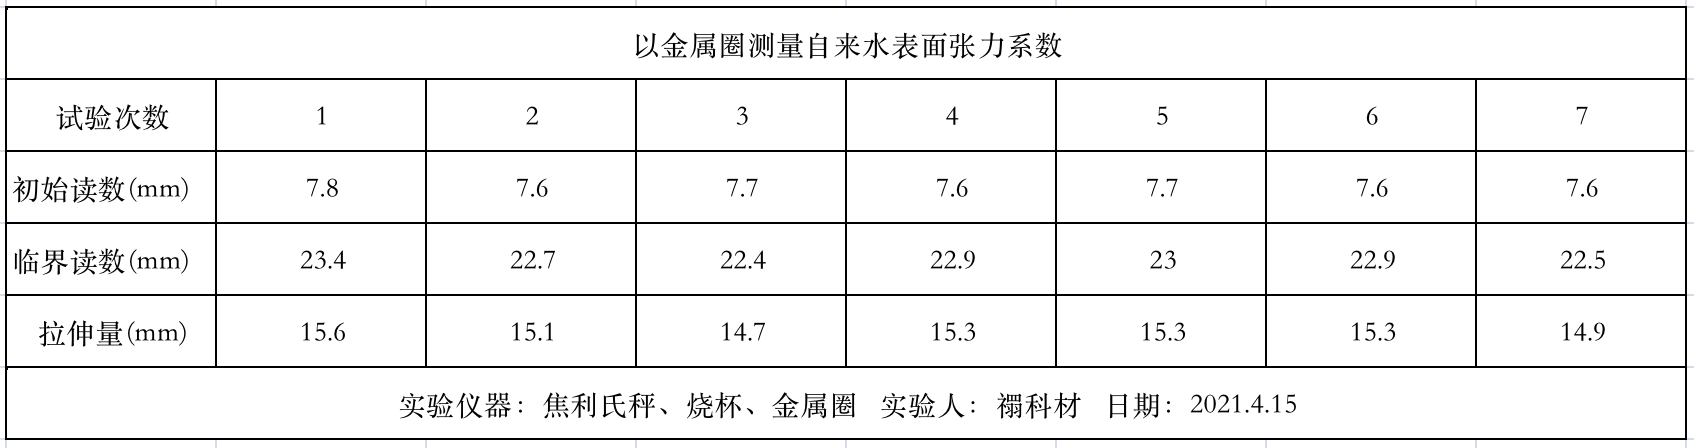
\includegraphics[width=13cm]{自来水.png}
    \end{figure}
        
    \begin{center}
        \emph{\\[0.01cm]\zihao{-4}金属丝测量不同浓度洗洁精}
    \end{center}

    \begin{figure}[ht]
        \centering 
        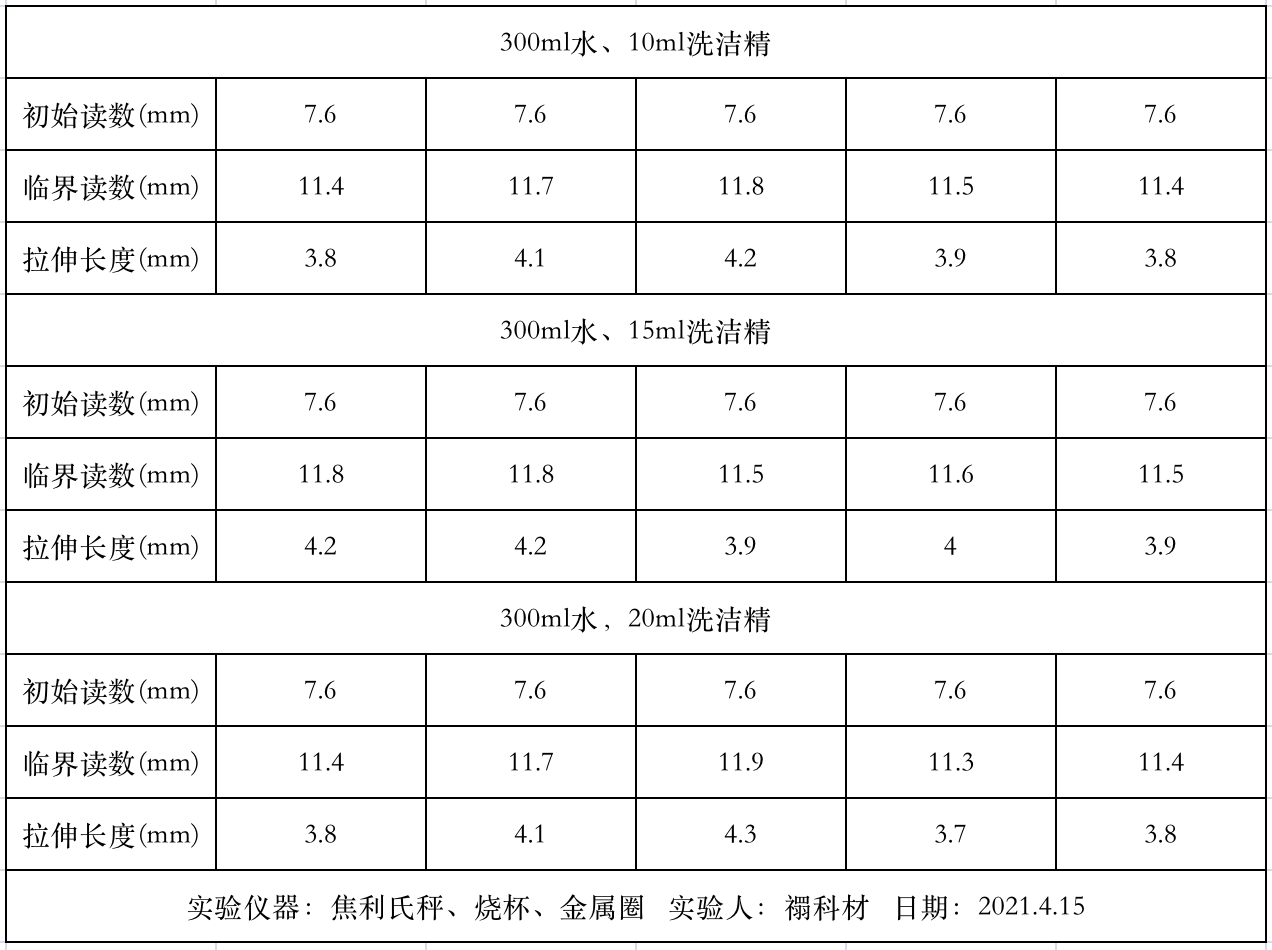
\includegraphics[width=13cm]{不同.png}
    \end{figure}

    \section{实验器材测量参数处理}

    \begin{center}
        \emph{\\[0.01cm]\zihao{-4}弹簧劲度系数的测量}
    \end{center}

    以弹簧形变量(mm)为X轴,所受拉力(mN)为Y轴作图,根据胡克定律,直线斜率即为弹簧劲度系数(N/m):

    \begin{figure}[ht]
        \centering 
        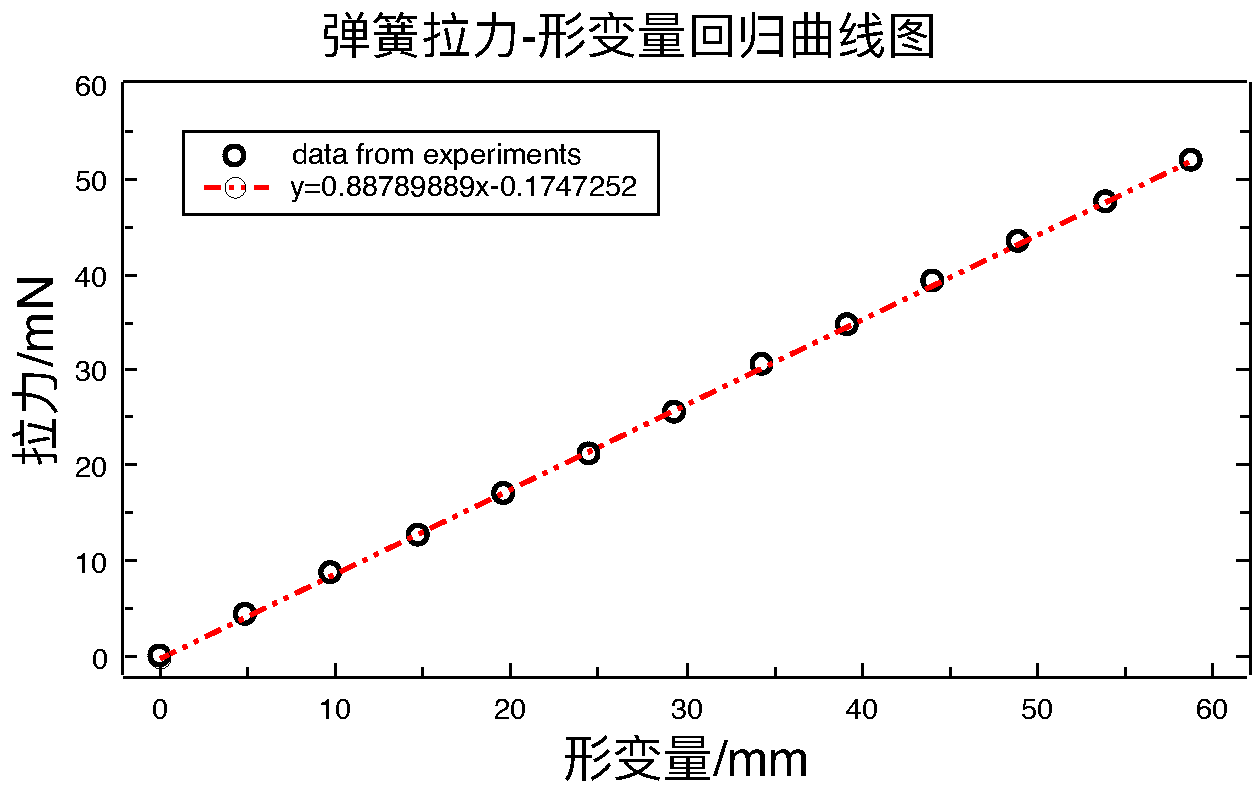
\includegraphics[width=13cm]{l.pdf}
    \end{figure}

    \begin{figure}[ht]
        \centering
        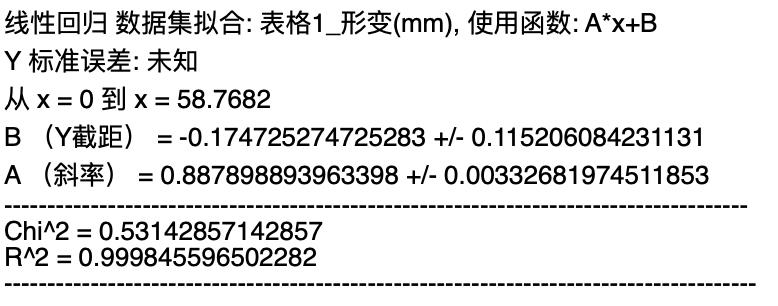
\includegraphics[width=10cm]{l1.png}
    \end{figure}

    由图可知,实验数据点基本落在拟合曲近旁,相关系数$R^2=0.999845$与1相近,表明拉力(mN)与形变量(mm)有很强的线性相关性,
    通过线性拟合计算弹簧劲度系数是合理可行的

    \emph{斜率$k$的标准差:}
    \begin{equation*}
        \sigma_k =k\sqrt{(\frac{1}{R^2}-1)/(n-2)}=0.88789889\sqrt{(\frac{1}{0.999845}-1)/(13-2)} =0.003326819 (N/m)
    \end{equation*}

    \emph{斜率$k$展伸不确定度:}
    \begin{equation*}
        U_{0.95}=t_p·\sigma_k=2.2·0.003326819=0.0073190034(N/m)
    \end{equation*}

    \emph{截距$b$标准差:}
    \begin{equation*}
        \sigma_b=\sqrt{\overline{{x^2}}}·\sigma_k=\sqrt{\frac{107.5^2+146.4^2+180.4^2+211.3^2+239.4^2+266.0^2}{13}}·0.003326819=0.11520608456(mN)
    \end{equation*}

    \emph{截距$b$展伸不确定度:}
    \begin{equation*}
        U_{0.95}=t_{0.95}·\sigma_b=2.2·0.11520608456=0.2534533860502(mN)
    \end{equation*}

    \emph{\zihao{-4}故弹簧劲度系数:}

    \begin{equation}
        k=0.8879±0.0073 (N/m)
    \end{equation}

    \begin{center}
        \emph{\\[0.01cm]\zihao{-4}金属丝长度}
    \end{center}

        \emph{长度$l$平均值:}
        \begin{equation*}
            \overline{l}=\frac{4.47	 +4.48+	4.48+	4.48+	4.48+	4.49	+4.48	+4.48}{8} =4.48(cm)
        \end{equation*}

        \emph{长度$l$标准差:}
        \begin{equation*}
            \sigma _l=\sqrt{\frac{\sum_{i=1}^8 (l_i-\overline{l})^2}{8-1}}=\sqrt{\frac{1.9998*10^{-4}}{7}}=0.005345(cm)
        \end{equation*}

        \emph{长度$A$类不确定度:}
        \begin{equation*}
            U_A=t_{0.95}\frac{\sigma_l}{\sqrt{n}}=2.36·\frac{0.005345}{\sqrt{8}}=0.00446(cm)
        \end{equation*}

        \emph{长度$B$类不确定度:}
        \begin{equation*}
            U_{B}=k_p·\frac{\varDelta B_仪}{C}=1.96·\frac{0.08}{3}=0.052267(cm)
        \end{equation*}

        \emph{长度$l$展伸不确定度(P=0.95):}
        \begin{equation*}
           U_{l}=\sqrt{U_A^2+U_B^2}= \sqrt{0.00446^2+0.052267^2}=0.052457(cm)
        \end{equation*}

        \emph{\zihao{-4}结果:}
        \begin{equation}
            l=4.48±0.052cm 
        \end{equation}
    


    \begin{center}
        \emph{\\[0.01cm]\zihao{-4}金属圈直径}
    \end{center}

    \emph{直径$d$平均值:}
    \begin{equation*}
        \overline{d}=\frac{3.71+	3.72+	3.66	+3.67+	3.69	+.68+	3.71+	3.65}{8} =3.68625(cm)
    \end{equation*}

    \emph{直径$d$标准差:}
    \begin{equation*}
        \sigma _d=\sqrt{\frac{\sum_{i=1}^8(d_i-\overline{d})^2}{8-1}}=\sqrt{\frac{4.58752*10^{-3}}{7}}=0.0256(cm)
    \end{equation*}

    \emph{直径$A$类不确定度:}
    \begin{equation*}
        U_A=t_{0.95}\frac{\sigma_d}{\sqrt{n}}=2.36·\frac{0.0256}{\sqrt{8}}=0.02136(cm)
    \end{equation*}

    \emph{直径$B$类不确定度:}
    \begin{equation*}
        U_B=k_p·\frac{\varDelta B_仪}{C}=1.96·\frac{0.08}{3}=0.052267(cm)
    \end{equation*}

    \emph{直径$d$展伸不确定度(P=0.95):}
    \begin{equation*}
       U_{d}=\sqrt{U_A^2+U_B^2}= \sqrt{0.02136^2+0.052267^2}=0.056463(cm)
    \end{equation*}

    \emph{\zihao{-4}结果:}
    \begin{equation}
        C=11.58±0.18cm 
    \end{equation}


    \section{表面张力系数测量数据处理}

    \begin{center}
        \emph{\\[0.01cm]\zihao{-4}金属丝测量洗洁精表面张力}
    \end{center}

    \emph{拉伸长度$h_1$平均值:}
    \begin{equation*}
        \overline{h_1}=\frac{3.5+	3.5	+3.7+	3.4	+2.8+	3.8	+3.4}{7} =3.442857 (mm)
    \end{equation*}

    \emph{拉伸长度$h_1$标准差:}
    \begin{equation*}
        \sigma _{h_1}=\sqrt{\frac{\sum_{i=1}^7(h_i-\overline{h})^2}{7-1}} =\sqrt{\frac{0.6171409}{6}}=0.320713(mm)
    \end{equation*}

    \emph{拉伸长度$A$类不确定度:}
    \begin{equation*}
        U_A=t_{0.95}\frac{\sigma_{h_1}}{\sqrt{n}}=2.45·\frac{0.320713}{7}=0.296985(mm)
    \end{equation*}

    \emph{拉伸长度$B$类不确定度:}
    \begin{equation*}
        U_B=k_p·\frac{\varDelta B_仪}{C}=1.96·\frac{0.1}{1.732}=0.113164(mm)
    \end{equation*}

    \emph{拉伸长度$h_1$展伸不确定度(P=0.95):}
    \begin{equation*}
       U_{h_1}=\sqrt{U_A^2+U_B^2}= 0.317815(mm)
    \end{equation*}

    \emph{\zihao{-4}结果:}
    \begin{equation*}
        h_1=3.44±0.32mm
    \end{equation*}

    \begin{equation*}
        \sigma = \frac{kh_1}{2l} = \frac{0.8879*3.44*10^{-3}}{2*4.48*10^{-2}} = 0.034089(N/m)
    \end{equation*}
    
    \emph{\zihao{-4}不确定度:}
    \begin{equation*}
        \frac{U_{\sigma}}{\sigma}=\sqrt{(\frac{U_{h_1}}{h_1})^2+(\frac{U_l}{l})^2+(\frac{U_k}{k})^2}=
        \sqrt{(\frac{0.32}{3.44})^2+(\frac{0.052}{4.48})^2+(\frac{0.0073}{0.8879})^2}= 0.0941 
    \end{equation*}

    \emph{\zihao{-4}最终结果:}
    \begin{equation}
        \sigma=0.0341±0.0031(N/m)
    \end{equation}



    \begin{center}
        \emph{\\[0.01cm]\zihao{-4}金属圈测量自来水表面张力}
    \end{center}

    \emph{拉伸长度$h_2$平均值:}
    \begin{equation*}
        \overline{h_2}=\frac{15.6	+15.1+	14.7+	15.3	+15.3+	15.3+	14.9}{7} =15.171429(mm)
    \end{equation*}

    \emph{拉伸长度$h_2$标准差:}
    \begin{equation*}
        \sigma _{h_2}=\sqrt{\frac{\sum_{i=1}^7 (h_i-\overline{h})^2}{7-1}}= \sqrt{\frac{0.534284}{6}} = 0.298408(mm)
    \end{equation*}

    \emph{拉伸长度$A$类不确定度:}
    \begin{equation*}
        U_A=t_{0.95}\frac{\sigma_{h_2}}{\sqrt{n}}=2.45·\frac{0.298408}{\sqrt{7}}=0.276330(mm)
    \end{equation*}

    \emph{拉伸长度$B$类不确定度:}
    \begin{equation*}
        U_B=k_p·\frac{\varDelta B_{h_2}}{C}=1.96·\frac{0.1}{1.732}=0.113164(cm)
    \end{equation*}

    \emph{拉伸长度$h_2$展伸不确定度(P=0.95):}
    \begin{equation*}
       U_{h_2}=\sqrt{U_A^2+U_B^2}=\sqrt{0.27633^2+0.113164^2}= 0.298604(mm)
    \end{equation*}

    \emph{\zihao{-4}结果:}
    \begin{equation*}
        h_2=15.17±0.30mm 
    \end{equation*}

    \begin{equation*}
        \sigma = \frac{kh_1}{2l} = \frac{0.8879*15.17*10^{-3}}{2*11.58*10^{-2}} = 0.0581582(N/m)
    \end{equation*}
    
    \emph{\zihao{-4}不确定度:}
    \begin{equation*}
        \frac{U_{\sigma}}{\sigma}=\sqrt{(\frac{U_{h_1}}{h_1})^2+(\frac{U_l}{l})^2+(\frac{U_k}{k})^2}=
        \sqrt{(\frac{0.30}{15.17})^2+(\frac{0.18}{11.58})^2+(\frac{0.0073}{0.8879})^2}= 0.026463
    \end{equation*}

    \emph{\zihao{-4}最终结果:}
    \begin{equation}
        \sigma=0.0582±0.0015(N/m)
    \end{equation}


    \begin{center}
        \emph{\\[0.01cm]\zihao{-4}金属丝测量不同浓度洗洁精}
    \end{center} 


    \begin{center}
        \emph{300ml水、10ml洗洁精:}
    \end{center}
 
    \emph{拉伸长度$h'_1$平均值:}
    \begin{equation*}
        \overline{h'_1}=\frac{3.8+	4.1	+4.2+	3.9	+3.8}{5} =3.960000(mm)
    \end{equation*}

    \emph{拉伸长度$h'_1$标准差:}
    \begin{equation*}
        \sigma _{h'_1}=\sqrt{\frac{\sum_{i=1}^5 (h_i-\overline{h})^2}{5-1}}= \sqrt{\frac{0.1319999}{4}}=0.181659(mm)
    \end{equation*}

    \emph{拉伸长度$A$类不确定度:}
    \begin{equation*}
        U_A=t_{0.95}\frac{\sigma_{h_2}}{\sqrt{n}}=2.78·\frac{0.181659}{\sqrt{5}}=0.225848(mm)
    \end{equation*}

    \emph{拉伸长度$B$类不确定度:}
    \begin{equation*}
        U_B=k_p·\frac{\varDelta B_{h_2}}{C}=1.96·\frac{0.1}{1.732}=0.113164(mm)
    \end{equation*}

    \emph{拉伸长度$h'_1$展伸不确定度(P=0.95):}
    \begin{equation*}
       U_{h'_1}=\sqrt{U_A^2+U_B^2}=\sqrt{0.225848^2+0.113164^2}=0.252613(mm)
    \end{equation*}

    \emph{\zihao{-4}结果:}
    \begin{equation*}
        h'_1=3.96±0.25mm 
    \end{equation*}

    \begin{equation*}
        \sigma = \frac{kh_1}{2l} = \frac{0.8879*3.96*10^{-3}}{2*4.48*10^{-2}} = 0.039242(N/m)
    \end{equation*}
    
    \emph{\zihao{-4}不确定度:}
    \begin{equation*}
        \frac{U_{\sigma}}{\sigma}=\sqrt{(\frac{U_{h_1}}{h_1})^2+(\frac{U_l}{l})^2+(\frac{U_k}{k})^2}=
        \sqrt{(\frac{0.25}{3.96})^2+(\frac{0.052}{4.48})^2+(\frac{0.0073}{0.8879})^2}= 0.06471
    \end{equation*}

    \emph{\zihao{-4}最终结果:}
    \begin{equation}
        \sigma=0.0392±0.0025(N/m)
    \end{equation}


    \begin{center}
        \emph{300ml水、15ml洗洁精:}
    \end{center}

    \emph{拉伸长度$h'_2$平均值:}
    \begin{equation*}
        \overline{h'_2}=\frac{4.2+	4.2	+3.9+	4+	3.9}{5} =4.040000(mm)
    \end{equation*}

    \emph{拉伸长度$h'_2$标准差:}
    \begin{equation*}
        \sigma _{h'_2}=\sqrt{\frac{\sum_{i=1}^5 (h_i-\overline{h})^2}{5-1}} = \sqrt{\frac{0.09200005}{4}}=0.151658(mm)
    \end{equation*}

    \emph{拉伸长度$A$类不确定度:}
    \begin{equation*}
        U_A=t_{0.95}\frac{\sigma_{h_2}}{\sqrt{n}}=2.78·\frac{0.151658}{\sqrt{5}}=0.188549(mm)
    \end{equation*}

    \emph{拉伸长度$B$类不确定度:}
    \begin{equation*}
        U_B=k_p·\frac{\varDelta B_{h_2}}{C}=1.96·\frac{0.1}{1.732}=0.113164(mm)
    \end{equation*}

    \emph{拉伸长度$h'_1$展伸不确定度(P=0.95):}
    \begin{equation*}
       U_{h'_2}=\sqrt{U_A^2+U_B^2}=\sqrt{0.188549^2+0.113164^2}=0.219902(mm)
    \end{equation*}

    \emph{\zihao{-4}结果:}
    \begin{equation*}
        h'_2=4.04±0.22mm 
    \end{equation*} 

    \begin{equation*}
        \sigma = \frac{kh_1}{2l} = \frac{0.8879*4.04*10^{-3}}{2*4.48*10^{-2}} = 0.040034(N/m)
    \end{equation*}
    
    \emph{\zihao{-4}不确定度:}
    \begin{equation*}
        \frac{U_{\sigma}}{\sigma}=\sqrt{(\frac{U_{h_1}}{h_1})^2+(\frac{U_l}{l})^2+(\frac{U_k}{k})^2}=
        \sqrt{(\frac{0.22}{4.04})^2+(\frac{0.052}{4.48})^2+(\frac{0.0073}{0.8879})^2}= 0.056282
    \end{equation*}

    \emph{\zihao{-4}最终结果:}
    \begin{equation}
        \sigma=0.0400±0.0022(N/m)
    \end{equation}



    \begin{center}
        \emph{300ml水、20ml洗洁精:}
    \end{center}
    \emph{拉伸长度$h'_3$平均值:}
    \begin{equation*}
        \overline{h'_3}=\frac{3.8	+4.1+	4.3	+3.7	+3.8}{5} =3.940000(mm)
    \end{equation*}

    \emph{拉伸长度$h'_3$标准差:}
    \begin{equation*}
        \sigma _{h'_3}=\sqrt{\frac{\sum_{i=1}^5 (h_i-\overline{h})^2}{5-1}} = \sqrt{\frac{0.2519999}{4}}=0.250998(mm)
    \end{equation*}

    \emph{拉伸长度$A$类不确定度:}
    \begin{equation*}
        U_A=t_{0.95}\frac{\sigma_{h_2}}{\sqrt{n}}=2.78·\frac{00.250998}{\sqrt{5}}=0.312054(mm)
    \end{equation*}

    \emph{拉伸长度$B$类不确定度:}
    \begin{equation*}
        U_B=k_p·\frac{\varDelta B_{h_2}}{C}=1.96·\frac{0.1}{1.732}=0.113164(mm)
    \end{equation*}

    \emph{拉伸长度$h'_1$展伸不确定度(P=0.95):}
    \begin{equation*}
       U_{h'_3}=\sqrt{U_A^2+U_B^2}=\sqrt{0.312054^2+0.113164^2}=0.331940(mm)
    \end{equation*}

    \emph{\zihao{-4}结果:}
    \begin{equation*}
        h'_3=3.94±0.33mm 
    \end{equation*}

    \begin{equation*}
        \sigma = \frac{kh_1}{2l} = \frac{0.8879*3.94*10^{-3}}{2*4.48*10^{-2}} = 0.039043(N/m)
    \end{equation*}
    
    \emph{\zihao{-4}不确定度:}
    \begin{equation*}
        \frac{U_{\sigma}}{\sigma}=\sqrt{(\frac{U_{h_1}}{h_1})^2+(\frac{U_l}{l})^2+(\frac{U_k}{k})^2}=
        \sqrt{(\frac{0.33}{3.94})^2+(\frac{0.052}{4.48})^2+(\frac{0.0073}{0.8879})^2}= 0.084956
    \end{equation*}

    \emph{\zihao{-4}最终结果:}
    \begin{equation}
        \sigma=0.0390±0.0033(N/m)
    \end{equation}

    \section{结果汇总}

    \begin{figure}[ht]
        \centering
        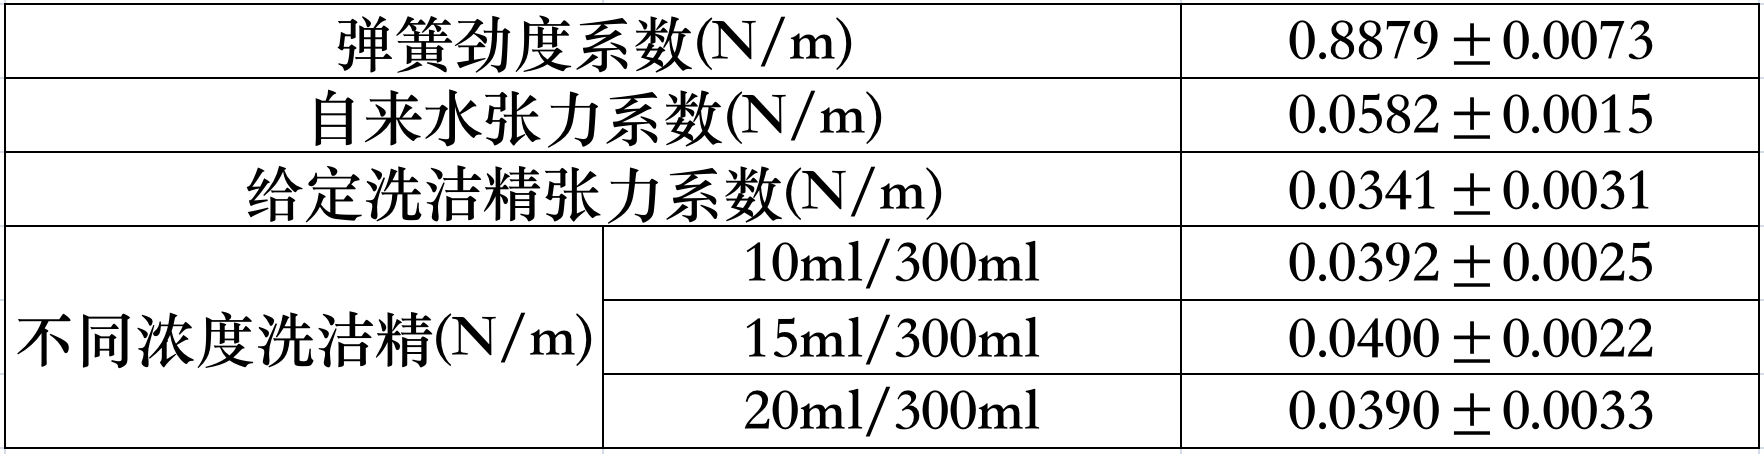
\includegraphics[width=13cm]{结果汇总.png}
    \end{figure}
    


    \section{误差分析}
    \zihao{-4}
    查询资料得知,清水表面张力系数为0.072(N/m),本实验中使用金属圈测得的张力系数偏小,分析有以下几点原因。

    (1)实验仪器的缺陷。为了始终保持三线对齐,操作者必须一边通过旋钮调节弹簧上端的拉伸长度,一边用手移动烧杯来实现。用手移动烧杯的过程中由于
    液体表面已经受到拉伸,很容易破裂;如果保持烧杯不动,就必须经过大量尝试,来寻找拉脱时恰好三线对齐的烧杯位置。由于液体的拉脱位置具有一定的随机性,可见这难度极大,也不科学合理。
    
    (2)实验环境的缺陷。实验过程中观察到如果液体没有稳定就开始实验,弹簧的临界长度是偏小的,这也合乎常理。然而如果液面有丝毫波动,都会对临界长度造成很大影响,有时差别甚至会达到0.5mm。
    这些微小扰动主要来自同学们的行走、言谈和邻桌同学较大幅度的操作,这也解释了结果的不确定度比较大的现象.

    (3)测量弹簧劲度系数时,观察到使用的砝码有所磨损,可能使得测量的劲度系数偏大

     由于洗洁精属于表面活性剂,浓度增加预计表面张力会减小。然而实验数据并没有显示出这种趋势,经分析有以下原因:

    (1)使用金属丝的过程中,由于金属丝的重心不处于悬挂点正下方,导致拉脱时金属丝两脚倾斜,一侧率先达到临界值而脱离液面。通过受力分析可知,金属丝受到的表面张力力矩不为0,张力作用线偏大,
    测得的洗洁精张力系数偏小

    (2)由于金属丝长度较金属圈短,受力只在一条线上,较金属圈更加不稳定,更容易受到外界干扰而提前拉脱,这个现象在实验中尤为明显。
    
    
    \section{提出改进}
    首先,实验设备必须改进。焦利氏秤只有一个旋钮,用来控制弹簧上端的拉伸,而通过三线对齐保证弹簧下端固定。
    这种设计看似合理,然而其中蕴含着极大的实验误差。为了保证三线对齐,拉伸弹簧时当小镜子刻度线高过玻璃管刻度线时
    便需要将烧杯下移以恢复对齐状态。由于液膜已被拉伸,此时如果徒手拧松螺丝、移动烧杯,势必造成液体扰动,导致提前拉脱,更加无法保证三线对齐,为提高测量精确度做出的努力前功尽弃。
    而为了减少这种徒手操作,尽量只用旋钮控制,操作者不得不进行大量的尝试。这也是本次实验的操作者为了改良实验技术而迟迟没有测出数据的主要原因。

    既然误差来源于实验器材的不合理设计,则必须改良,从根本上减少误差。设想有两个旋钮的焦利氏秤,一个控制弹簧上端高度,一个控制烧杯高度,支架透明。实验过程中通过平衡两个旋钮,能在极大程度上
    保证三线始终对齐,而两旋钮对应刻度的差即是所求的弹簧拉伸量。

    其次,实验应在安静人少的地方进行。如误差分析中所述,同学们走路时产生的振动传递到烧杯水面上就会减小表面的稳定性,导致提前拉脱。老师测量的标准数据大概是一个人测得的。

    再次,实验所用的铁丝的重心要尽量处在中心位置,如果有所倾斜,则铁丝一端达到临界时另一端没有临界,会造成实验数据偏小的后果

    \section{思考题}
    
    \emph{\\[0.02cm]\zihao{-4}1.焦利氏秤法测定液体的表面张力有什么优点?}

    (1)焦利氏秤是在测量过程中保持下端固定在某一位置,靠上端的位移大小来称衡,保证了实验的精确度

    (2)锥形弹簧的设计减小了弹簧劲度系数的系统误差

    (3)标尺最小分度为$0.1mm$,有利于测量微小形变,提高液膜破裂时受力的准确度

    (4)直接测量表面张力的大小,无需间接使用公式计算,减少实验步骤,也不需要不确定度传递

    \emph{\\[0.2cm]\zihao{-4}2. 焦利氏秤的弹簧为什么做成锥形?}

    做成锥形是为了消除弹簧自重对劲度系数测量的实验误差,提高实验精确度

    \emph{\\[0.2cm]\zihao{-4}3. 拉托法测定液体表面张力系数存在哪些误差?}

    (1)实验原理方面,将圆圈或者铁丝提出水面时,两侧液面其实和水平面夹角并不是绝对的$\frac{\pi}{2}$,偏差一个小角度$\theta $,而由于近似处理,导致张力测量值偏小,实际$\sigma $偏大

    (2)实验过程方面,已分析如上


    \nocite{shiyanjiaocheng}
    \nocite{daolun}
    \bibliography{math}

\end{document}

